\documentclass{article}
\usepackage{amsmath}
\usepackage{amssymb}
\usepackage{fancyhdr}
\usepackage{booktabs}

\usepackage[T1]{fontenc}
\usepackage[utf8]{inputenc}
\usepackage{regexpatch}
\makeatletter
\usepackage{letltxmacro}
\usepackage{aligned-overset}

\usepackage{hyperref}
\usepackage{cleveref}

\usepackage{nowidow}
\usepackage{microtype} 
\usepackage{siunitx}

\usepackage{titling}
\usepackage{braket}
\usepackage{minted}
\usepackage[margin=1in]{geometry}
\usepackage[super]{nth}

\setlength\parindent{0pt}

\title{CMSC32700 Project Report: Verifying Wiesner's quantum money using SQIR}
\author{Adrian E. Lehmann}
\date{Jun 4, 2021}

\begin{document}

\maketitle

\section{Introduction}
At the moment we have many quantum circuit designs, for transmitting and encoding information but none of them have been tried to be verified using SQIR~\cite{SQIR}. 
Hence in this project we will try to verify a simple $n$-qubit quantum key distribution protocol ``Wiesner's quantum money''~\cite{wiesner} which we will examine close in \cref{sec:wiesner}. 
We will then proceed to prove a few interesting properties of the scheme.
The mechanization of said proofs will be described in \cref{sec:proof-impl}.

\section{Background}

\subsection{Coq, QWIRE, SQIR}
To formally verify the algorithm we will be using a quantum formal verification stack based on the Coq proof assistant~\cite{Coq}.
On top of Coq, there are two main libraries that we will be using: QWIRE~\cite{QWIRE} and SQIR~\cite{SQIR}.
QWIRE is a quantum programming language that has been embedded into Coq and SQIR is a fromal verification framework built on top of QWIRE.
While SQIR was originally intended as an intermediate representation for a verified quantum compiler (VOQC~\cite{voqc}), it has been used to prove various algorithms, such as Deutsch-Josza's~\cite{deutsch} or Shor's~\cite{shor} algorithm.


\subsection{Wiesner's qunatum money}\label{sec:wiesner}

Wiesner's quantum money proposed by Stephen Wiesner in 1983~\cite{wiesner}, is a quantum verification scheme that intends to encode an $n$ bit integer. 
Given two parties, Alice and Bob, Alice will encode the n bit integer by choosing a basis such that each bit of the integer will either be encoded to quantum in the basis $\ket{0}, \ket{1}$ or the basis $\ket{-},\ket{+}$.
Physically this corresponds to a choice of polarization rotated by \ang{45}.
Bob will then decode the integer using his basis.
Using the no-cloning property, it follows that when Bob measures to get the classical information, he will certainly get the correct output if his basis is equal to Alice's.
If his basis does not match, he will have a chance of $\frac{1}{2^{n_{\text{diff}}}}$ getting the correct result, where $n_{\text{diff}}$ is the number of bits his basis differs from Alice's.
It follows that Bob's chance getting the correct output at random is $(\frac{3}{4})^n$.

In the context of money, the $n$-bit integer would be a serial number, Alice the central bank, and Bob a malicious \nth{3} party trying to copy money.
The central bank can validate bills with a given serial numbers, whil the \nth{3} party would be unable to decode the bill to get a valid serial number to copy.

\section{Proof Implementation}\label{sec:proof-impl}
We implement a proof to show that Wiesner's quantum money scheme for any $n$ qubits will yield the correct state with probability $1$, if Alice and Bob have the same base, and will only yield the correct output with probability $(\frac{1}{2})^{n_{\text{diff}}}$ when Alice's and Bob's bases are different, where $n_{\text{diff}}$ is the number of bits that are different two bases. In the following, we will discuss the steps we took to prove these conjectures. The accompanying code can be found on GitHub\footnote{\url{https://github.com/adrianleh/SQIR/blob/main/examples/Wiesner.v} - we use commit \texttt{6dd2e57} for line-\#s in snippets}.

\subsection{Circuit design}

Our circuit will operate on each qubit independently (i.e. one qubit only influeces the ouput of itself, and the circuit does not require any ancilla), where each qubit will have a Pauli $X$-Gate classically controlled by a data bit, followed by two Hadamard gates, clasically controlled by Alice's and Bob's basis bits.

Given an input of $\ket{0}$, this will if the data bit is $1$, transform to $\ket{1}$, and then use Alice's basis bit to either stay in the basis $\ket{0},\ket{1}$ basis, or rotate into the $\ket{+},\ket{-}$ basis. 
Bob's basis bit will then control the rotation bob applies to attempt to restore the original basis.

We will now proceed to describing the circuit for $n$ qubits. 
For this we will assume, we have $3$ $n$-sized arrays $data, ab, bb$, containing classical data, basis bits for Alices, and basis bits for Bob respectively.

We designed the circuit inductively, row by row using, such that for our circuit is defined as
$$C(n) = \begin{cases}
I_1&, n=0\\
C(n-1) \otimes R(n)&, n>0
\end{cases}$$,
where $R$ is the function constructing a row
$$R(n) = \begin{cases}X&, data[n] = 1\\ I_2&, \text{else}\end{cases} \times \begin{cases}H&, ab[n] = 1\\ I_2&, \text{else}\end{cases} \times \begin{cases}H&, bb[n] = 1\\ I_2&, \text{else}\end{cases}$$

This is implemented in Coq by the definitions \texttt{circuit'\_qubit\_\_non\_meas} ($\hat{=} R(n)$) and \texttt{circuit'}.

An implementation note is that instead of tensoring the constructed unitaries, we chose to append unitaries of dimension $n$, where we solely padded the unitaries to move our operations to the correct qubit.

The Coq implementation of this can be seen in \cref{fig:Coq-circuit}.

We can see the resulting construction in \cref{fig:circuit}.
\begin{figure}[h]
    \centering
    \begin{minted}[linenos,tabsize=1,breaklines]{Coq}
Notation bit_string := (list bool). (* line 19 *)
Notation combined_bit_string := (list (bool * bool * bool)) (* line 20 *). 

Definition alice_bit_manip (base : bool) (data : bool) (n i : nat) : base_ucom n := (* line 79 *)
  (if data then X i else SKIP);
  (if base then H i else SKIP).
Definition bob_bit_manip (base : bool) (n i : nat) : base_ucom n := (* line 92 *)
  if base then H i else SKIP.
Definition circuit'_qubit_i_non_meas (ad ab bb : bool) (n i : nat) : base_ucom n := (* line 104 *)
  alice_bit_manip ab ad n i; bob_bit_manip bb n i.

 
Fixpoint circuit'_helper (l : combined_bit_string) (n : nat) (i : nat) : base_ucom n := (* line 106 *)
  match l with
    | [] => SKIP
    | ((ad,ab),bb)::l' => circuit'_helper l' n (S i); circuit'_qubit_i_non_meas ad ab bb n i
  end.
    
Definition circuit' (alice_data alice_base bob_base : bit_string) (n : nat) := (* line 122 *)
  circuit'_helper (zip (zip alice_data alice_base) bob_base) n 0.
    \end{minted}
    \caption{The QWIRE definition for our circuit}
    \label{fig:Coq-circuit}
\end{figure}



\begin{figure}[h]
    \centering
    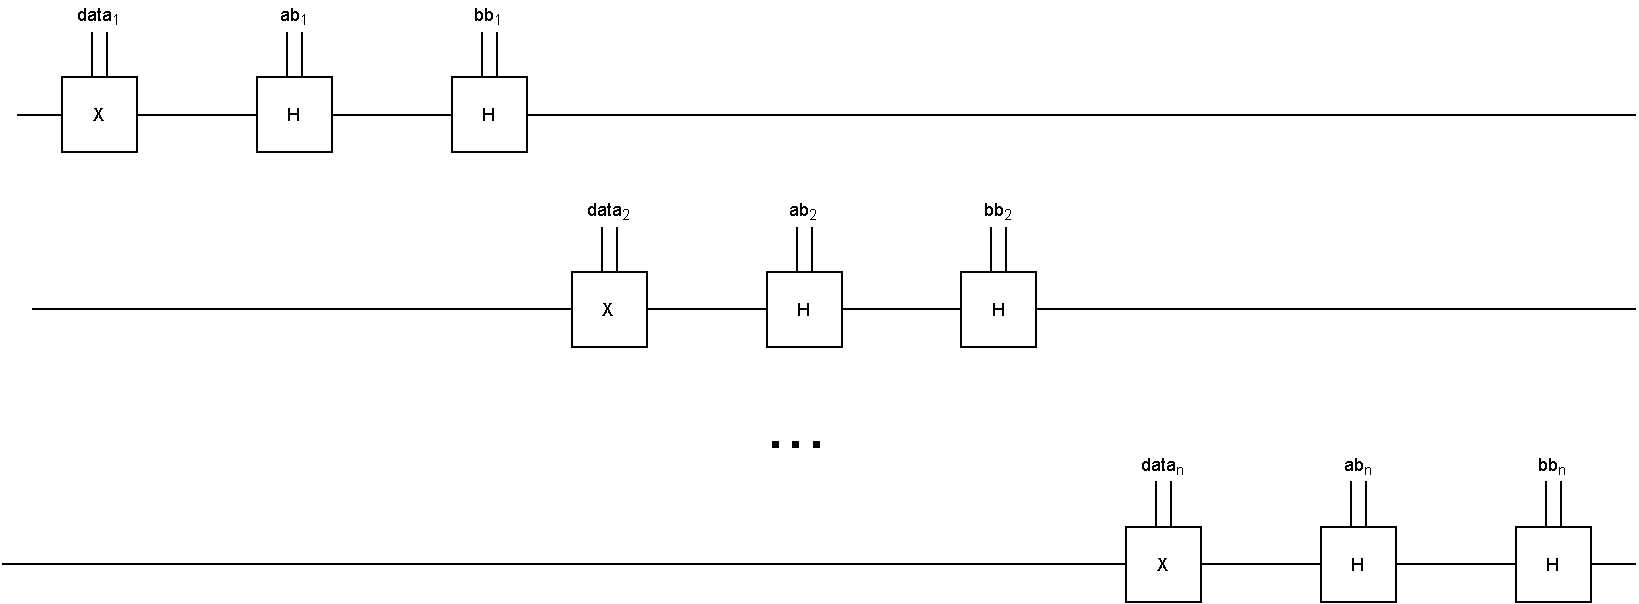
\includegraphics[width=\textwidth]{res/Wiesner.pdf}
    \caption{Wiesner's quantum money for $n$ qubits}
    \label{fig:circuit}
\end{figure}

While some algorithms in other SQIR examples use $n$ qubits and use the library feature \texttt{npar} to replicate their circuits, we cannot use this, since each qubit of our circuit depeneds on different classical controls and is hence not identical. This fact will complicate our proof and cause us to require the work of \cref{sec:circuit-growth}.


Henceforth we will assume the input to the circuit is initialized to $\ket{\underbrace{0...0}_n}$.

We note that this design is our second iteration, where in the first iteration instead of grouping operations by qubit, we tried grouping them by type (i.e., grouping all the $X$, all of Alice's Hadamard gates, and all of Bob's Hadamard gates) and then concatenating but that turned out to make proof more difficult. The construction of this circuit is still included in the source file (\texttt{circuit}) for the sake of documentation.

\subsection{Individual qubit correctness}\label{sec:qubit-correct}
We prove that for any individual qubit our construction yields 
$Q(data,ab,bb) = \begin{cases} 
\ket{0}&, data=0 \wedge ab=bb\\
\ket{1}&, data=1 \wedge ab=bb\\
\ket{-}&, data=0 \wedge ab \neq bb\\
\ket{+}&, data=1 \wedge ab \neq bb
\end{cases}
$

This proof basically follows directly from the definitions of Pauli $X$ and Hadamard, and the self-inverse property of Hadamard.

In our implementation we prove this through the four lemmata, one for each of the cases listed above:
%\footnote{\texttt{circuit'\_individual\_qubit\_non\_meas\_\{same,diff\}\_base\_\{true,false\}} in code on lines $138,157,172,185$ respectively}:
\begin{minted}[linenos,tabsize=1,breaklines,escapeinside=||,mathescape=true]{Coq}
Lemma circuit'_individual_qubit_non_meas_same_base_false: forall base n i, (n > 0)%nat -> (i < n)%nat -> uc_eval (circuit'_qubit_i_non_meas false base base n i) = I (2 ^ n). (* line 138 *)
Lemma circuit'_individual_qubit_non_meas_same_base_true: forall base n i, (n > 0)%nat -> uc_eval (circuit'_qubit_i_non_meas true base base n i) = @pad 1 i n σx.  (*line 157*)
Lemma circuit'_individual_qubit_non_meas_diff_base_false: forall base_a base_b n i, base_a <> base_b -> (n > 0)%nat -> uc_eval (circuit'_qubit_i_non_meas false base_a base_b n i) = @pad 1 i n hadamard. (* line 172 *)
Lemma circuit'_individual_qubit_non_meas_diff_base_true: forall base_a base_b n i, base_a <> base_b -> (n > 0)%nat -> uc_eval (circuit'_qubit_i_non_meas true base_a base_b n i) = @pad 1 i n (hadamard |$\times$| σx). (* line 185 *)

\end{minted}
Though we note that the actual Coq lemma prove that the implementation yields gates that trivally transform $\ket{0}$ into said states, instead of proving states directly. 
This proof-design was chosen as operations on unitaries are easir to work with in future steps.

\subsection{Inductive circuit growth}\label{sec:circuit-growth}

Likely the most important, yet most challenging lemma to prove was about circuit growth, in the inductive proof that we will see in \cref{sec:circuit-correct}, we will need to able to reason about growing circuits.
Specifically, we will require the following theorem:
\begin{minted}[linenos,tabsize=1,breaklines,escapeinside=||,mathescape=true]{Coq}
Theorem circuit'_helper_growth: forall n l, (length l = S n) ->  uc_eval(circuit'_helper l (S (S n)) 1) =  I 2 |$\otimes$| uc_eval (circuit'_helper l (S n) 0). (* line 1164 *)
\end{minted}
which essentially says for any $n>0$ building step $1$ in the inductive construction of a circuit of size $n+1$, the current step is equal to tensoring $I_2$ to the \nth{0} step in building a circuit of size $n$.

Though proving this theorem by itself turned out to be impossible and we resorted to proving a stronger notion where we prove that for a circuit and $n>0$ of size $n+i$, the evaluation of the circuit at step $i+1$ is equal to $I_{i+1}$ tensored with the evaluation of the \nth{0} step of a circuit with size $n$
\begin{minted}[linenos,tabsize=1,breaklines,escapeinside=||,mathescape=true]{Coq}
Lemma circuit'_helper_growth_i: forall n l i, (length l = S n) -> uc_eval(circuit'_helper l ((S i) + (S n)) (S i)) =  I (2^(S i)) |$\otimes$| uc_eval (circuit'_helper l (S n) 0). (* line 277 *)
\end{minted}

The reason we note this property is because this is how we were able to inductively reason about a heterogenous circuit of size $n$ which had been inductively defined.
This theorem is the foundation of any useful reasoning about this circuit.

We note that this circuit growth lemma could likely be generalized to all circuits consisting solely of unitary gates each controlled by a classical bit, where each qubit operates independently, and the circuit itself is defined by the same structure of inductive definition. 
Though this generalization had to be forgone in the interest of time and the questionable applicability to other problems.

Further, a potentially general-enough-to-be-extracted lemma that we used in the process is:
\begin{minted}[linenos,tabsize=1,breaklines,escapeinside=||,mathescape=true]{Coq}
Lemma kron_dist_mult_id : forall n m (B C : Square m) , (I n) |$\otimes$| (B |$\times$| C) = ((I n) |$\otimes$| B) |$\times$| ((I n) |$\otimes$| C). (* line 266 *)
\end{minted}
\subsection{Inductive circuit correctness}\label{sec:circuit-correct}
Our goal is to prove that given any data and any bases that our algorithm yields we expected output.

We define our expected output inductively as follows:
$$O(n,data,ab,bb) = \begin{cases}I_1&,n=0\\ Q(data[n],ab[n],bb[n]) \otimes O(n-1, data, ab,bb)&, n>0\end{cases}$$

To prove this correct we shall proceed inductively. Our base case has been shown in \cref{sec:qubit-correct}.

To perform the inductive step we will separate the new added qubit from the remaining construction and then using our inductive circuit growth property, we will show that given individual qubit correctness the entire circuit is correct.

The synopsis of the relevant Coq code can be seen in \cref{fig:correct-main-circuit}
\begin{figure}[h]
    \centering
\begin{minted}[linenos,tabsize=1,breaklines,escapeinside=||,mathescape=true]{Coq}
Definition q_bool (b : bool) := if b then |$\ket{1}$| else |$\ket{0}$| (* line 231 *).

Definition output_state_qubit_i (d ab bb : bool) := (* line 242 *)
  if (eqb ab bb) then
    q_bool d
  else
    hadamard |$\times$| q_bool d.

Fixpoint output_state n (l : combined_bit_string) : Vector (2 ^ n) := (* line 248 *)
  match l with
  | [] => I 1
  | (d, ab, bb)::l' => output_state_qubit_i d ab bb |$\otimes$| output_state (n-1) l'
  end.
  
Theorem circuit'_output_correct: forall n data ab bb, (length data = S n) -> (length ab = S n) -> (length bb = S n) -> (uc_eval (circuit' data ab bb (S n))) |$\times$| initial_state (S n) = output_state (S n) (zip (zip data ab) bb). (* line 1173 *)
\end{minted}
    \caption{Synopsis of relevant Coq statements for correctness}
    \label{fig:correct-main-circuit}
\end{figure}

\subsection{Individual qubit probability}\label{sec:qubit-prob}

What we can now prove using the construction of the indivdual qubits in \texttt{output\_state\_qubit\_i} (as seen in \cref{fig:correct-main-circuit}) that given $ab=bb$ we get upon measurement the expected result with certainty.
Whereas, if $ab\neq bb$, we can use the properties of hadamard to easily show we get the expected outputwith probability $\frac{1}{2}$.

In our implementation these facts are proven using the following two theorems:
\begin{minted}[linenos,tabsize=1,breaklines,escapeinside=||,mathescape=true]{Coq}
Theorem probability_correct_single_qubit: forall data base, probability_of_outcome (output_state_qubit_i data base base) (target_state_qubit_i data) = 1. (*line 1908*)

Theorem probability_incorrect_single_qubit: forall data ab bb, (ab <> bb) -> probability_of_outcome (output_state_qubit_i data ab bb) (target_state_qubit_i data) = (1/2)%R. (* line 1934 *)
\end{minted}

\subsection{Inductive circuit probability}\label{circuit-prob}
Using the fact that from \cref{sec:circuit-correct}, that we now have a vector representation of our evaluation, we can now prove facts about the execution without requiring deep circuit manipulation.

Using the definition of \texttt{output\_state} (as seen in \cref{fig:correct-main-circuit}), we can easily prove that our circuit yields our target state with probability $1$. 
Our target state hereby is defined as what we would intuitively expect:
$$T(n,data) = \begin{cases}
I_1&, n =0\\
\begin{cases}
\ket{1}&, data[n] = \texttt{true}\\
\ket{0}&, data[n] = \texttt{false}
\end{cases} \otimes T(n-1,data)&, n>0
\end{cases}$$

Using the fact that $T(n,data)$ is always a unit vector we can then prove certainty of correct output inductively using SQIR's lemma \texttt{probability\_of\_outcome\_is\_norm}, and a lemma to extract the newly added element from the resulting norm \texttt{norm\_kron}\footnote{This is another lemma that seems generally useful and could be extracted}. 

The other, perhaps more challenging undertaking was to show that given any two bases, the probability of getting \texttt{target\_state} upon measurement is $(\frac{1}{2})^{n_{\text{diff}}}$, where $n_{\text{diff}}$ is the number of non equal bits in the two bases. To prove this, we use the facts we established in \cref{sec:qubit-prob}, using the same lemmata as in the proof for equal bases to inductively prove the our conjecture.

The relevant Coq code for this section can be seen in \cref{fig:circuit-prob}.

\begin{figure}[H]
    \centering
\begin{minted}[linenos,tabsize=1,breaklines,escapeinside=||,mathescape=true]{Coq}

Notation target_state_qubit_i := q_bool. (* line 233 *)

Fixpoint target_state n (data: bit_string) : Vector (2^n) := (* line 235 *)
  match data with
  | [] => I 1
  | d::data' => target_state_qubit_i d |$\otimes$| target_state (n-1) data'
  end.
  
Theorem circuit'_same_base_correct: forall n data base, (length data = S n) -> (length base = S n) -> (uc_eval (circuit' data base base (S n))) |$\times$| initial_state (S n) = target_state (S n) data. (* line 1792 *)

Lemma target_state_norm: forall n data, (length data = S n) -> norm ((target_state (S n) data)|$\dagger$| |$\times$| (target_state (S n) data)) = 1. (* line 1865 *)

Lemma norm_kron: forall (A : Vector 1) (B : Vector 1), @norm (1) (A |$\otimes$| B) = (@norm 1 A * @norm 1 B)%R. (* line 1799 *)

Lemma probability_of_outcome_is_norm : forall {d} (|$\phi$| |$\psi$| : Vector d),
  probability_of_outcome |$\phi$| |$\psi$| = ((norm (|$\phi\dagger \times \psi$|)) ^ 2)%R. (* Part of SQIR/examples/Utilities.v *)

Theorem probibility_correct: forall n data base, (length data = S n) -> (length base = S n) -> probability_of_outcome (uc_eval (circuit' data base base (S n)) |$\times$| initial_state (S n)) (target_state (S n) data) = 1%R. (* line 1900 *)

Theorem probibility_incorrect: forall n n_diff data ab bb, (length data = S n) -> (length ab = S n) -> (length bb = S n) -> count_diff ab bb = n_diff -> probability_of_outcome (uc_eval (circuit' data ab bb (S n)) |$\times$| initial_state (S n)) (target_state (S n) data) = ((1/2)%R^n_diff)%R. (* line 2081 *)
\end{minted}
    \caption{Synopsis of Coq code from statements about probability}
    \label{fig:circuit-prob}
\end{figure}

\bibliographystyle{IEEEtran}
\bibliography{bib}

\end{document}
